\chapter{Análisis y Diseño}

Las etapas iniciales de la metodología ``Cascada'' consisten en el análisis y diseño previos al inicio de la implementación del producto final. Es importante que estas fases sean completadas en su totalidad para que el desarrollo sea éxitoso. Este proyecto se plantea para ser diseñado y desarrollado en un tiempo de 50 dias hábiles calendario y la distribución del tiempo se define segun la complejidad de las tareas que implican cada fase.

\section{Análisis}
Para el diseño de un sistema de video-vigilancia inteligente es necesario tener en cuenta los elementos primordiales que lo componen. En este caso los principales módulos llegan a ser:
\begin{itemize}
    \item Visualizador de fotogramas.(Simulador de cámara)
    \item Servidor TCP (Servicio que aplica el protocolo TCP/IP)
    \item Servidor HTTP (Servicio que aplica el protocolo de la Web)
    \item Módulo SMTP (Módulo de envio de correo electrónico)
\end{itemize}

A continuación se detalla el funcionamiento esperado del sistema de video-vigilancia intelegente. El módulo de visualización es el más importante dado que es el encargado de capturar los fotogramas por medio de un lente físico que trabaje como cámara. Las

Referenciando a la figura \ref{fig:camera_screen}.
\begin{figure}[H]
    \begin{center}
        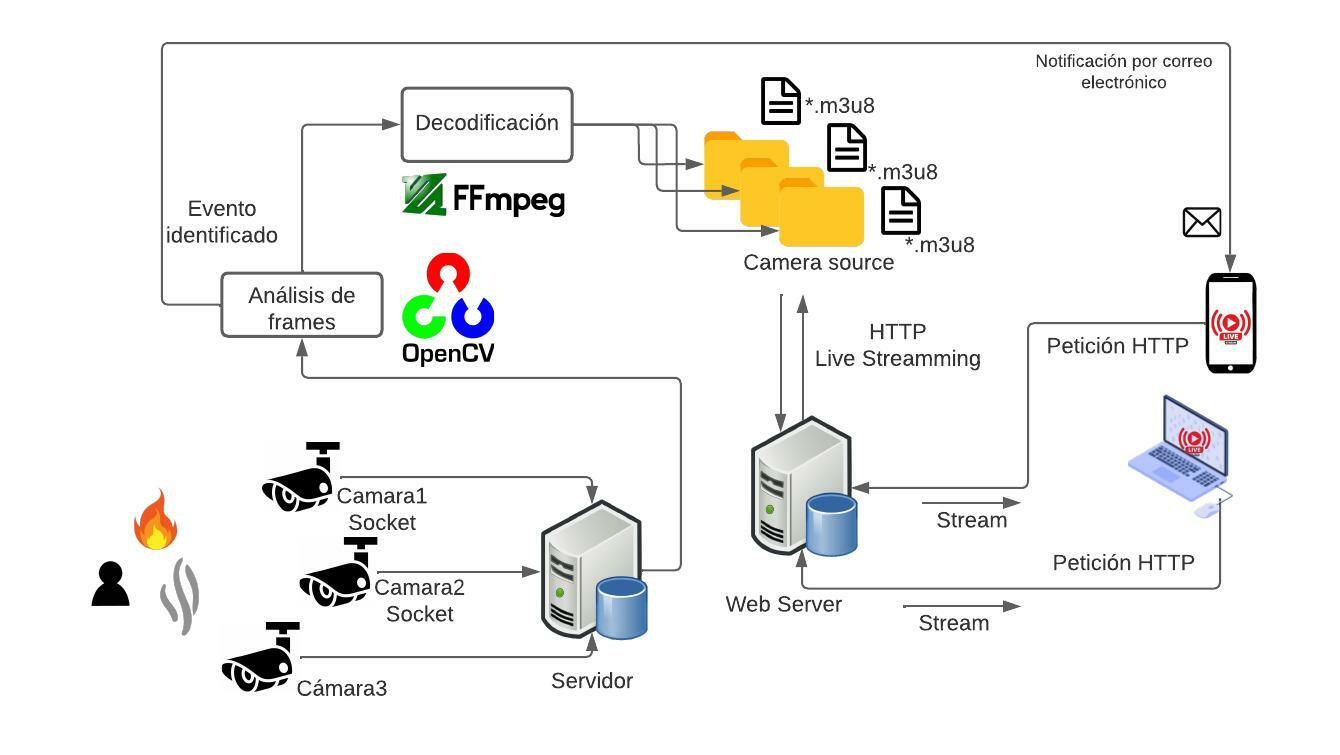
\includegraphics[width=15cm]{img/capitulo_4/main.jpeg}
        \caption{Diagrama de Gannt.}
        Fuente : Elaboración propia
        \label{fig:webcamera}
    \end{center}
\end{figure}

\subsection{Definición de Requerimientos}
Para la identificación de los requerimientos, se plantean los criterios de partida a tomar en cuenta en el diseño del sistema de video-vigilancia inteligente:
\begin{itemize}
    \item Costos altos en infraestructura de transmisión de video en vivo.
    \item Las características de identificación automática, estan disponibles para sistemas de video-vigilancia de alto nivel.
    \item Una alerta inmediata puede minimizar el impacto de alguna situación que ponga en peligro la integridad de bienes materiales y humanos.
    \item Los usuarios finales son personas que a menudo dejan su hogar para salir a trabajar, y usan constamente su correo electrónico.
\end{itemize}


\subsubsection{Requerimientos Funcionales}

\subsubsection{Requerimientos No Funcionales}

\section{Diseño}

\subsection{Diseño de clases}

\subsection{Diseño de interfaces}

\subsection{Diseño de consola de servidor}

\subsection{Diseño de entidad-relación (Base de datos)}

\subsection{Diseño de notificación}

\subsection{Diseño de interacción}

\subsection{Diagrama de interacción Cámara-Servidor}


\subsection{Requerimientos del sistema}
En esta fase es necesario delimitar el alcance y las capacidades del sistema planteado para la realización de la planificación inicial, estimación de tiempos, diseño y desarrollo. Para ello se define la lista inicial de requerimientos del sistema de video-vigilancia inteligente.\\

\begin{table}[H]
    \caption{Lista de requerimientos}
    \label{tabla:ejemplo}
    \begin{center}
        \begin{tabular}{ |c|l|} 
            \hline
            1. & Capturar fotogramas por medio de una o varias cámaras portatiles.\\ \hline
            2. & Visualizar los fotogramas capturados en tiempo real (captura de video).\\  \hline
            3. & Ejecutar el servicio de análisis y procesamiento de los fotogramas capturados.\\  \hline
            4. & Enviar los fotogramas capturados por medio de la red al servicio encargado de su análisis.\\ \hline
            5. & Permitir la recepción de fotogramas de varias fuentes hacia el servicio.\\ \hline
            6. & Transmitir los fotogramas convertidos en video en vivo desde fuentes diferentes.\\ \hline
            7. & Detectar movimiento a partir de los fotogramas recibidos desde distintas fuentes.\\ \hline
            8. & Detectar silueta humana a partir de los fotogramas recibidos desde distintas fuentes.\\ \hline
            9. & Notificar al usuario por medio de un correo electrónico cuando se de una detección.\\ \hline
        \end{tabular}
    \end{center}
    \begin{center}
        Fuente: Elaboración propia.
    \end{center}
\end{table}

\begin{table}[H]
    \caption{Tabla de planificación de las diferentes fases del modelo Cascada}
    \label{tabla:ejemplo}
    \begin{center}
        \begin{tabular}{|c|l|c|c|c|}
            \hline
            \textbf{Num.} & \textbf{Fase}  &  \textbf{Fecha inicial} & \textbf{Fecha final} & \textbf{Duración (días)}\\ \hline
            \textbf{1.} & Fase de requerimientos        & 6-jun        & 17-jun        & 10        \\ \hline
            \textbf{2.} & Fase de diseño del sistema       & 20-jun        & 8-jul        & 15        \\ \hline
            \textbf{3.} & Fase de implementación        & 11-jul        & 19-ago        & 30        \\ \hline
            \textbf{4.} & Fase de pruebas        & 22-ago         &   2-sep     &    10     \\ \hline
            \textbf{5.} & Fase de mantenimiento        & 5-sep        & 9-sep        & 5        \\ \hline
        \end{tabular}
        Fuente: Elaboración propia.
    \end{center}
\end{table}

\section{Identificación de Requerimientos del Sistema}
Referenciando a la figura \ref{fig:gannt}.
\begin{figure}[H]
    \begin{center}
        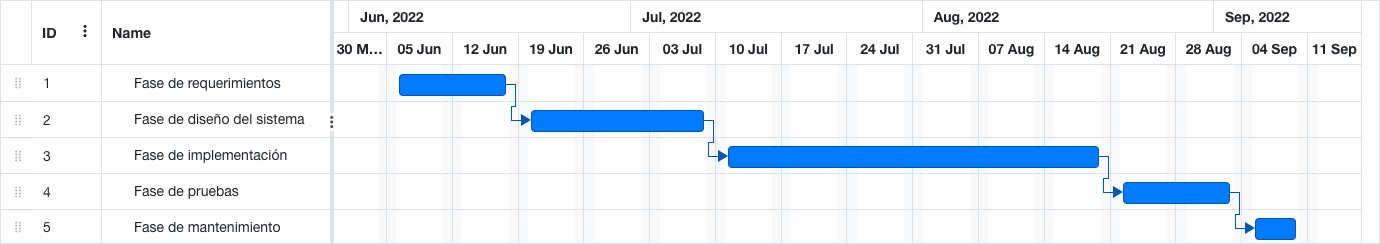
\includegraphics[width=17cm]{img/capitulo_4/gant.png}
        \caption{Diagrama de Gannt.}
        Fuente : Elaboración propia
        \label{fig:gannt}
    \end{center}
\end{figure}





Referenciando a la figura \ref{fig:camera_screen}.
\begin{figure}[H]
    \begin{center}
        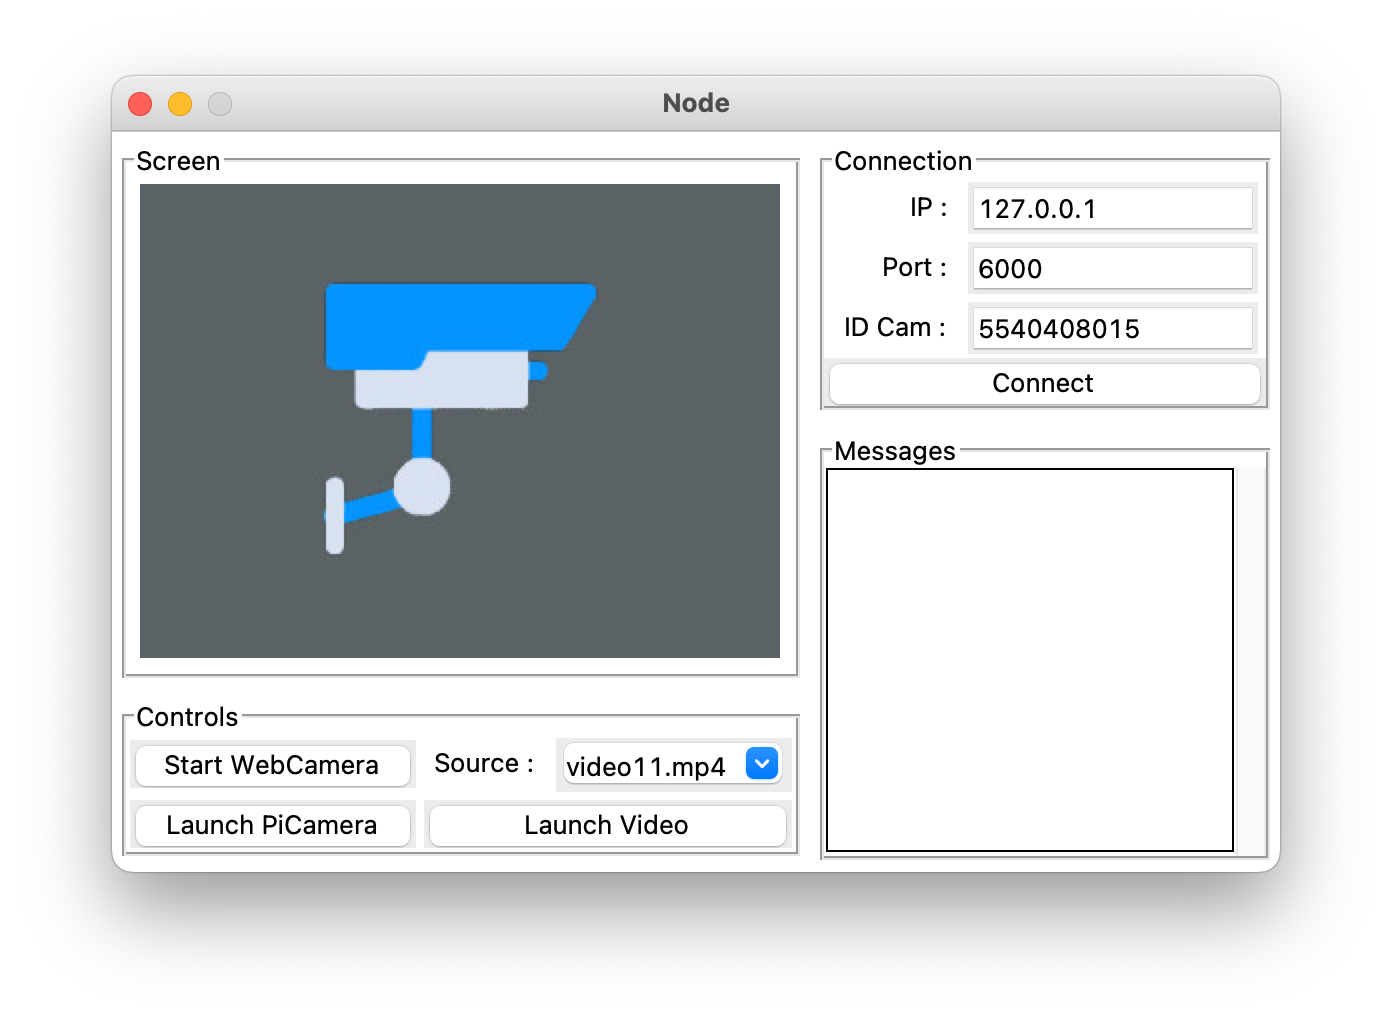
\includegraphics[width=13cm]{img/capitulo_4/camera_screen.png}
        \caption{Interfaz de la camara desarrollada.}
        Fuente : Elaboración Propia.
        \label{fig:camera_screen}
    \end{center}
\end{figure}

Referenciando a la figura \ref{fig:camera_screen}.
\begin{figure}[H]
    \begin{center}
        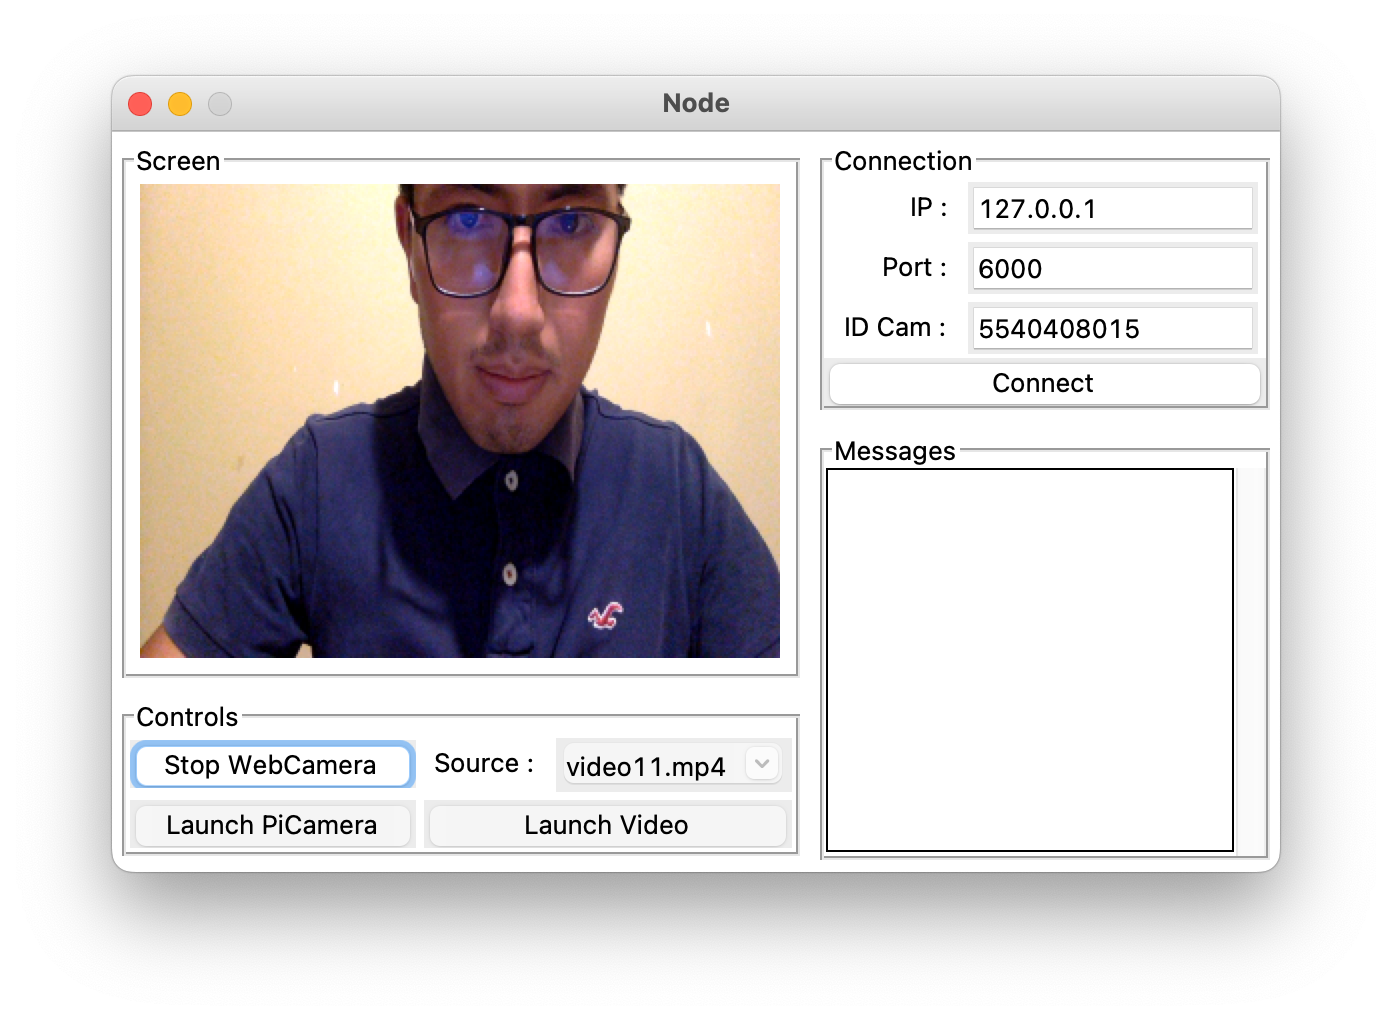
\includegraphics[width=13cm]{img/capitulo_4/webcamera.png}
        \caption{Diagrama de Gannt.}
        Fuente : Elaboración propia
        \label{fig:webcamera}
    \end{center}
\end{figure}

Referenciando a la figura \ref{fig:securityvideo}.
\begin{figure}[H]
    \begin{center}
        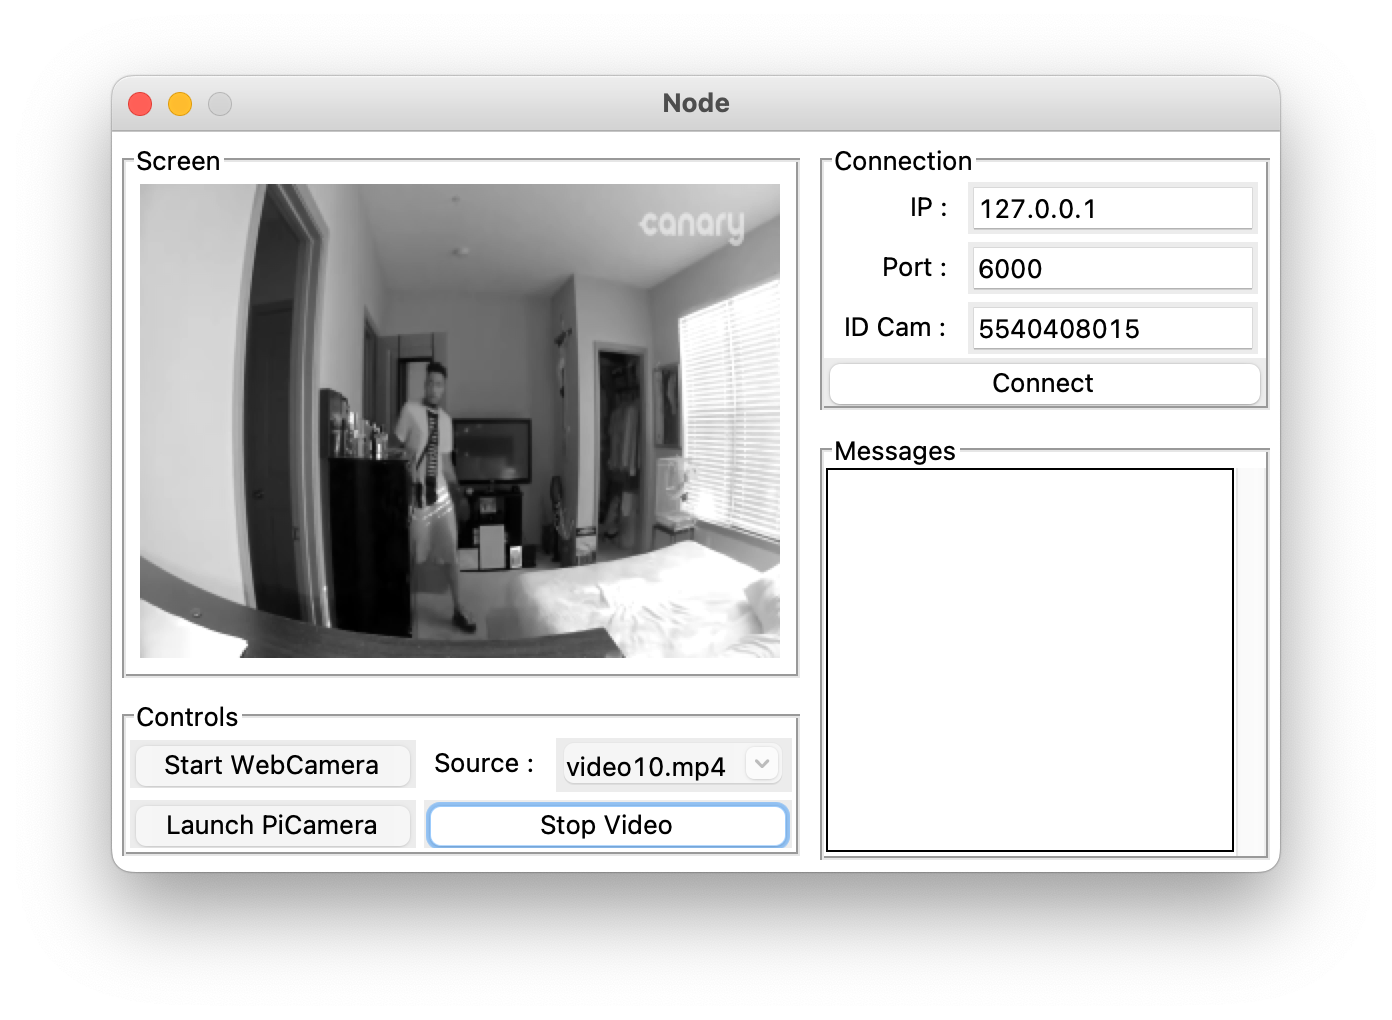
\includegraphics[width=13cm]{img/capitulo_4/security-video.png}
        \caption{Diagrama de Gannt.}
        Fuente : Elaboración propia
        \label{fig:securityvideo}
    \end{center}
\end{figure}

Referenciando a la figura \ref{fig:servertcp_console}.
\begin{figure}[H]
    \begin{center}
        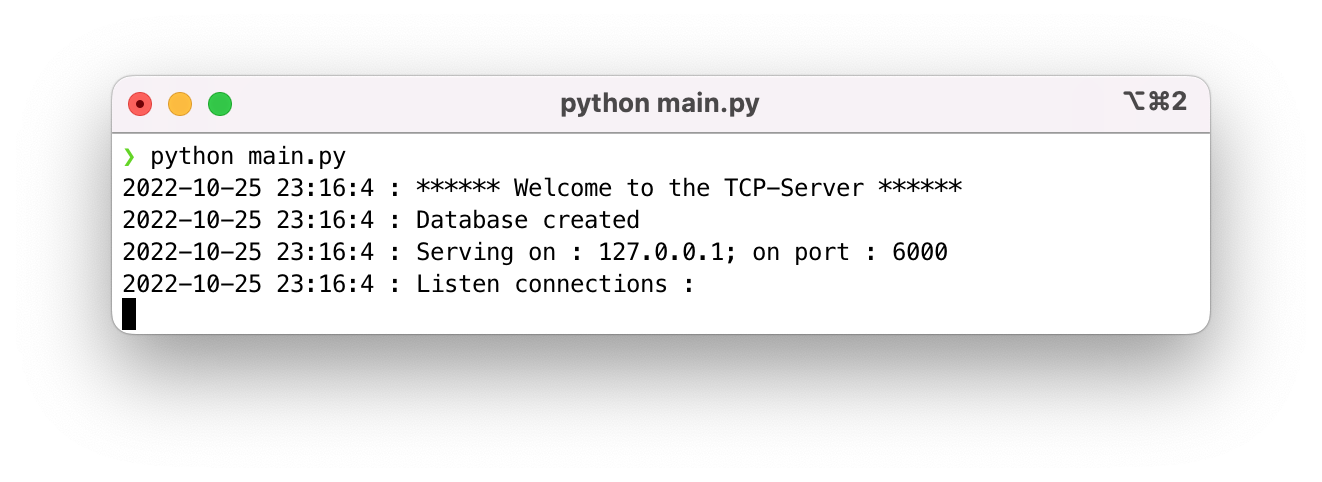
\includegraphics[width=15cm]{img/capitulo_4/tcp_server.png}
        \caption{Ejecución del servidor TCP.}
        Fuente : Elaboración propia
        \label{fig:servertcp_console}
    \end{center}
\end{figure}

\begin{center}
    \begin{tabular}{ |c|c|c|c| } 
    \hline
    \textbf{col1} & \textbf{col2} & \textbf{col3} \\
    \hline
    \multirow{3}{4em}{Multiple row} & cell2 & cell3 \\ 
    & cell5 & cell6  \\
    & cell8 & cell9 \\ 
    \hline
    \end{tabular}
\end{center}

\begin{center}
    \begin{tabular}{ |c|c| } 
     \hline
     1. & Requerimiento uno\\
     \hline 
     2. & Requerimiento dos \\ 
     \hline
     3. & Requerimiento tres \\ 
     \hline
    \end{tabular}
\end{center}

\subsection{Requerimientos del software}

\section{Análisis}
\section{Diseño de Módulos}

\begin{table}[H]
    \caption{Detalle de las pruebas realizadas}
    \label{tabla:ejemplo}
    \begin{center}
        \begin{tabular}{c|c|c|c|}
            \cline{2-4}
            & \textbf{Columna 1} & \textbf{Columna 2} & \textbf{Columna 3} \\ \hline
            \multicolumn{1}{|c|}{\textbf{Fila 1}} & item               & item               & item               \\ \hline
            \multicolumn{1}{|c|}{\textbf{Fila 2}} & item               & item               & item               \\ \hline
            \multicolumn{1}{|c|}{\textbf{Fila 3}} & item               & item               & item               \\ \hline
        \end{tabular}
    \end{center}
    Nota. Extraída de Apellido, N. (2000) \textit{Nombre del libro}.
    Editorial o universidad que lo publicó.
\end{table}

% \usepackage{cellspace}
% \setlength\cellspacetoplimit{4pt}
% \setlength\cellspacebottomlimit{4pt}
% \newcommand\cincludegraphics[2][]{\raisebox{-0.3\height}{\includegraphics[#1]{#2}}}
% \begin{table}[H]
%     \caption{Detalle de las pruebas realizadas}
%     \begin{center}
%         \begin{tabular}{|>{\centering}p{0.3\textwidth}|>{\centering}m{0.3\textwidth}|m{0.3\textwidth}<{\centering}|} 
%             \hline
%             \textbf{Columna 1} & \textbf{Columna 2} & \textbf{Columna 3} \\
%             \hline
%             \begin{minipage}{.3\textwidth}
%                 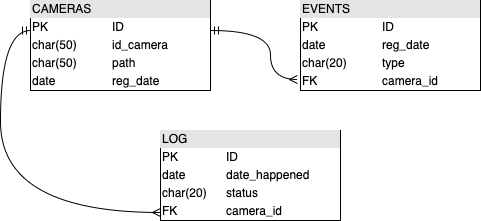
\includegraphics[width=\linewidth]{img/capitulo_4/db.png}
%             \end{minipage}& lorem lorem lorem lorem lorem lorem lorem lorem lorem lorem lorem lorem lorem lorem lorem lorem lorem lorem lorem lorem lorem
%             & \begin{itemize} 
%                 \item Remote delivery 
%                 \item Immersive experiences
%                 \item text proved
%             \end{itemize} \\ 
%             \hline
%             \begin{minipage}{.3\textwidth}
%                 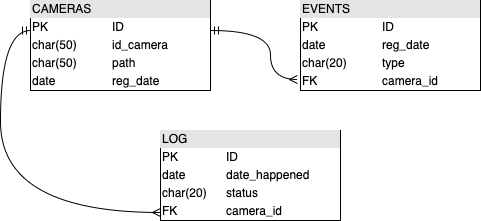
\includegraphics[width=\linewidth]{img/capitulo_4/db.png}
%             \end{minipage} & cell8 & \begin{itemize} 
%                 \item Remote delivery 
%                 \item Immersive experiences
%                 \item text proved
%             \end{itemize} \\
%             \hline
%         \end{tabular}
%     \end{center}
% \end{table}

\begin{table}[H]
    \caption{Detalle de las pruebas realizadas}
    \begin{center}
        \begin{tabular}{|>{\centering}p{0.6\textwidth}|m{0.3\textwidth}<{\centering}|} 
            \hline
            \textbf{Columna 1} & \textbf{Columna 3} \\
            \hline
            \begin{minipage}{.3\textwidth}
                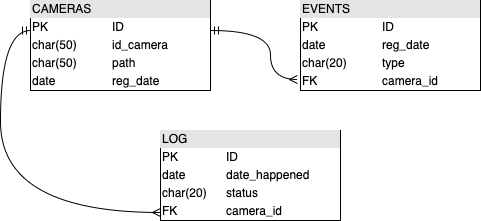
\includegraphics[width=\linewidth, height=40mm]{img/capitulo_4/db.png}
            \end{minipage}
            & \begin{itemize} 
                \item Remote delivery 
                \item Immersive experiences
                \item text proved
            \end{itemize} \\ 
            \hline
            \begin{minipage}{0.6\textwidth}
                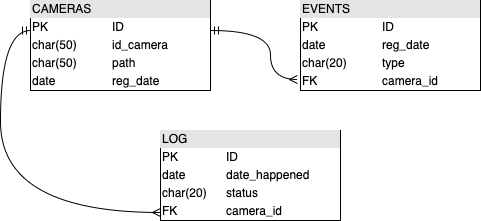
\includegraphics[width=\linewidth]{img/capitulo_4/db.png}
            \end{minipage} & \begin{itemize} 
                \item Remote delivery 
                \item Immersive experiences
                \item text proved
            \end{itemize} \\
            \hline
        \end{tabular}
    \end{center}
\end{table}


\begin{table}[H]
    \caption{Detalle de las pruebas realizadas}
    \label{tabla:ejemplo}
    \begin{center}
        \begin{tabular}{c|c|c|c|}
            \cline{2-4}
            & \textbf{Columna 1} & \textbf{Columna 2} & \textbf{Columna 3} \\ \hline
            \multicolumn{1}{|c|}{Fila 1 }& item             & item               & item               \\ \hline
            \multicolumn{1}{|c|} {Fila 2} & {item}               & item               & item               \\ \hline
            \multicolumn{1}{|c|} {Fila 3} & {item}              & item               & item               \\  \hline
        \end{tabular}
    \end{center}
    Nota. Extraída de Apellido, N. (2000) \textit{Nombre del libro}.
    Editorial o universidad que lo publicó.
\end{table}

\section{Identificación de Subsistemas}

Referenciando a la figura \ref{fig:ejemplo}.
\begin{figure}[H]
    \begin{center}
        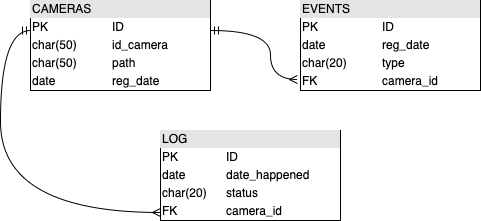
\includegraphics[width=10cm]{img/capitulo_4/db.png}
    \end{center}
    \caption{Ilustración de un ladrón}
    Fuente: Adaptada de Apellido, N. (2000) \textit{Nombre del libro}.
    Editorial o universidad que lo publicó.
    \label{fig:ejemplo}
\end{figure}

Referenciando a la figura \ref{fig:ejemplo}.
\begin{figure}[H]
    \begin{center}
        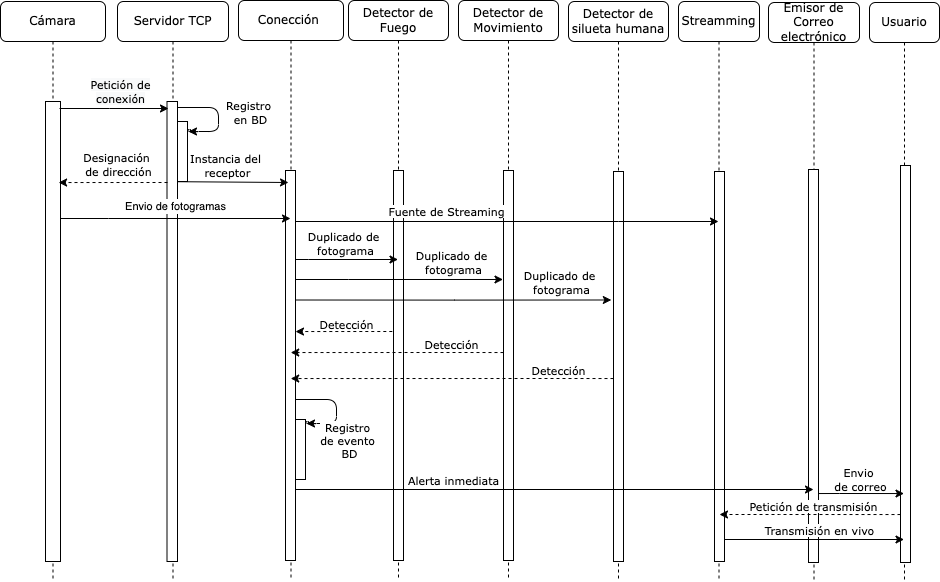
\includegraphics[width=18cm]{img/capitulo_4/interaccion.png}
    \end{center}
    \caption{Ilustración de un ladrón}
    Fuente: Adaptada de Apellido, N. (2000) \textit{Nombre del libro}.
    Editorial o universidad que lo publicó.
    \label{fig:ejemplo}
\end{figure}
\section{Comunicación de Sistemas}

\subsection{Sockets}

\section{Planificación}
